\documentclass{beamer}
\usepackage{ dsfont }
\usepackage[utf8]{inputenc}
\usepackage{minted}
\usepackage[english]{babel}
\setbeamersize{text margin left=10pt, text margin right=10pt} %new code
\usepackage{graphicx}
\usepackage{float}
\usepackage{subcaption}
\usepackage{wasysym}
\usefonttheme{professionalfonts} % using non standard fonts for beamer
\setbeamerfont{frametitle}{series=\bfseries}
\usepackage{animate}
\usepackage{movie15}
\usepackage{breqn, bm}
\usepackage{amsmath}
\usepackage[skins]{tcolorbox}
\usepackage{subcaption}

\definecolor{notgreen}{RGB}{255,127,0}
\definecolor{green}{RGB}{49,150,3}
\setbeamerfont{headline}{size=\small}


%----------------------------------------------------------------------------------------
%	 Package
%----------------------------------------------------------------------------------------
\usepackage{color}
\usepackage{url}
\beamertemplatenavigationsymbolsempty
\definecolor{cadmiumred}{rgb}{0.8, 0.8, 0.8}

%----------------------------------------------------------------------------------------
%	 Presentation settings
%----------------------------------------------------------------------------------------

\usetheme{default}
\usecolortheme{default}

\setbeamertemplate{itemize items}[triangle] 
\setbeamertemplate{enumerate items}[default]
 
\title[Variational Drop Out]{
	Data Mining In Action Course\\ 
	\vspace{1cm}
	\textbf{\textcolor{black}{Introduction in Deep Learning}}}

\author{Ashuha Arseniy$^{1, 2}$}
\institute[Bayesgroup, MIPT]{
	Bayesian Research Group$^1$, MIPT$^2$\\
	
	\medskip
	
\includegraphics[scale=0.5]{./img/logo} 
\includegraphics[scale=0.12]{./img/mipt}
	
	\href{ars-ashuha.ru/slides}{ars-ashuha.ru/slides}}

\date{\today}

\newcommand{\Expect}{\mathsf{E}}
\newcommand{\MExpect}{\mathsf{M}}
\newcommand{\cov}{\mathsf{cov}}
\setbeamertemplate{section in toc}[circle]

\addtobeamertemplate{navigation symbols}{}{%
	\usebeamerfont{footline}%
	\usebeamercolor[fg]{footline}%
	\hspace{1em}%
	\insertframenumber/\inserttotalframenumber
}


\begin{document}
\begin{frame}
	\titlepage 
\end{frame}

\begin{frame}{Cat vs Dogs}	
	\begin{center}
		  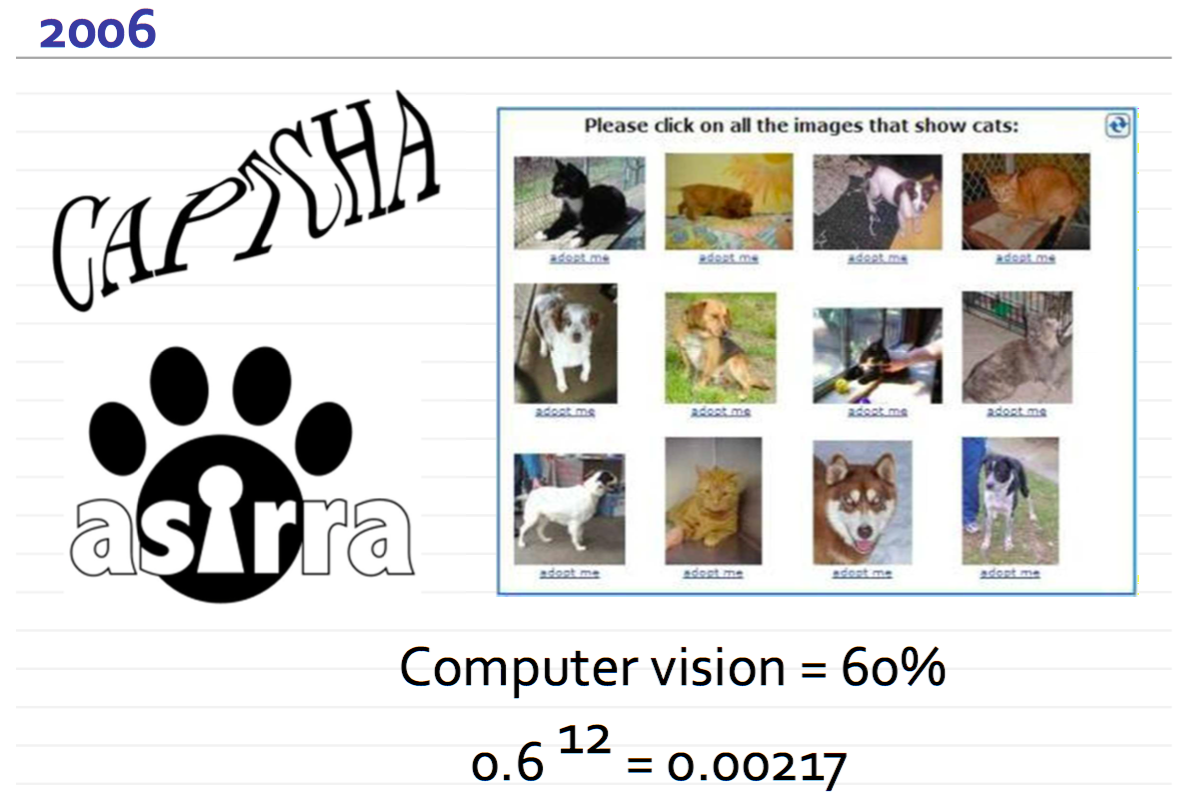
\includegraphics[scale=0.14]{img/cd1}	
		  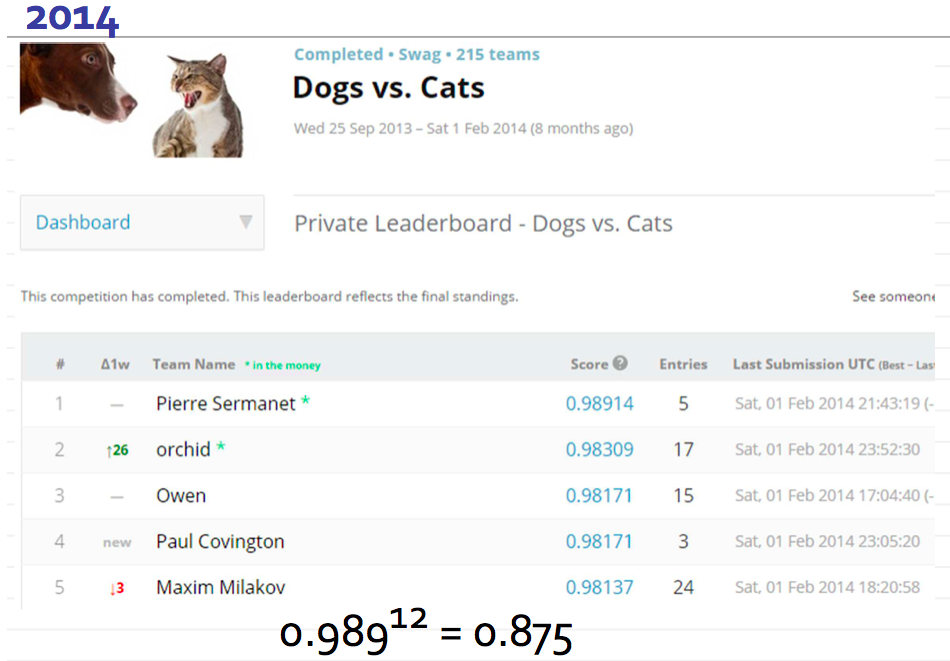
\includegraphics[scale=0.17]{img/cd2}	
		
		 
\includegraphics[scale=0.17]{img/cd3}	
	\end{center}
	  slides credit: prof.V. Lempitsky
\end{frame}

\begin{frame}{Motivation}	
 	\begin{itemize}
 		  \item We know that linear model is awesome 
	 	  \item Linear Models
		 	\begin{center}
		 		  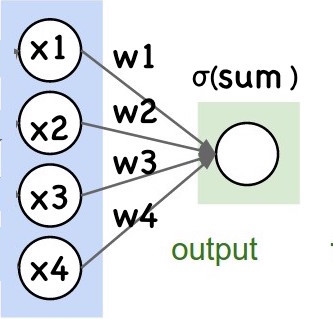
\includegraphics[scale=0.2]{img/nnn1}	
		 	\end{center}
 		  \item But LM describe our data bad course linearity 
	 	  \item Neural Nets
		 \begin{center}
	 			 	  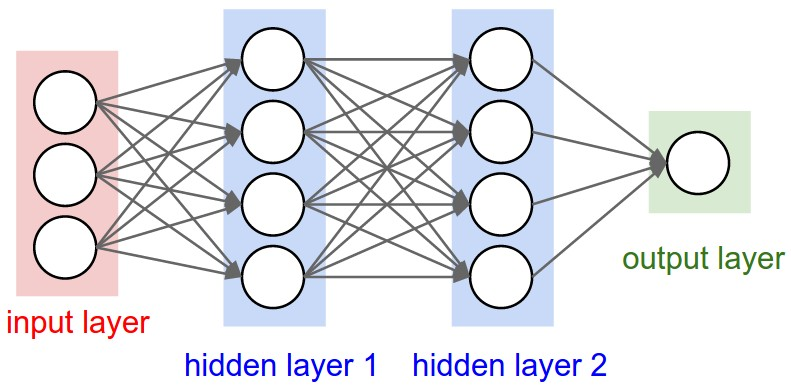
\includegraphics[scale=0.2]{img/nnn2}	
		 \end{center}
 	\end{itemize}
\end{frame}

\begin{frame}{Linear Models}
		 \begin{center}
		 	  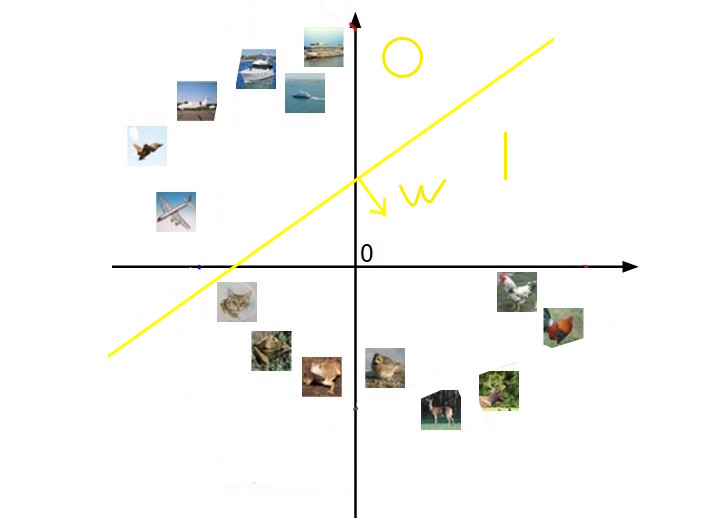
\includegraphics[scale=0.27]{img/pclf1}
		 	 
			   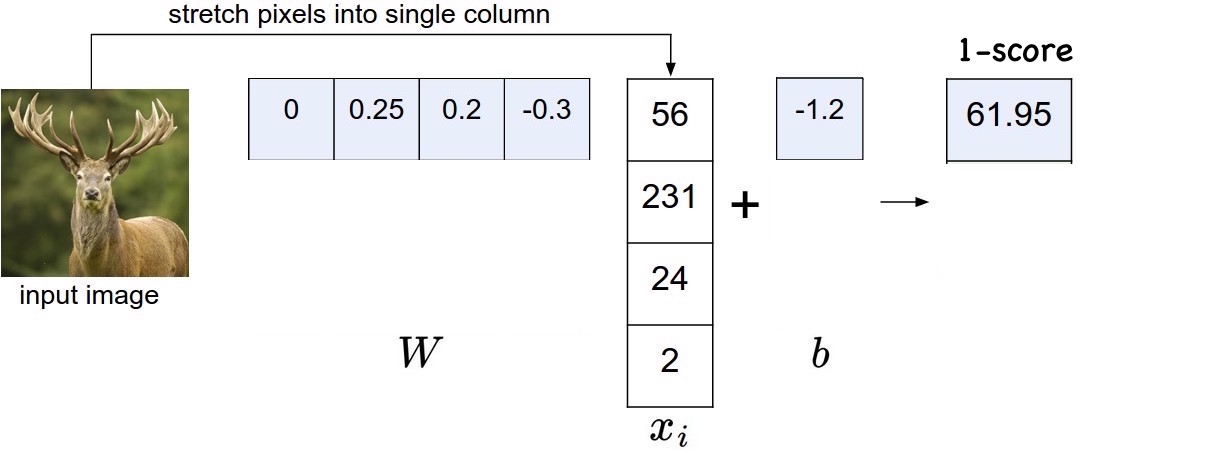
\includegraphics[scale=0.15]{img/clf1}
		 \end{center}
\end{frame}

\begin{frame}{Linear Models}
	\begin{center}
		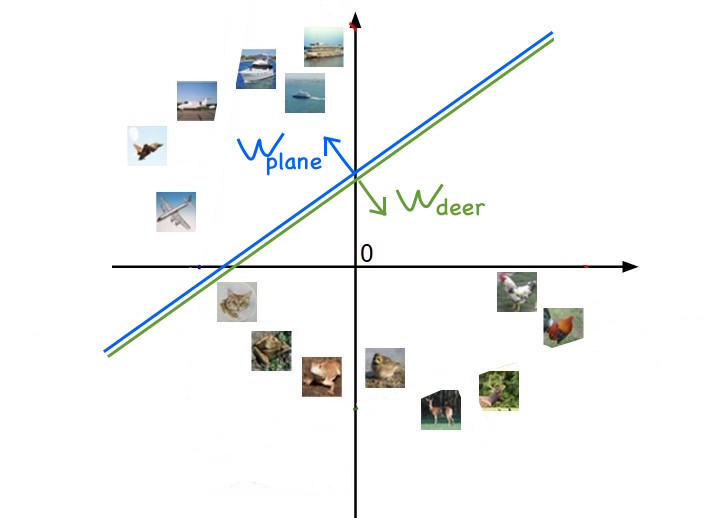
\includegraphics[scale=0.27]{img/pclf2}
		
		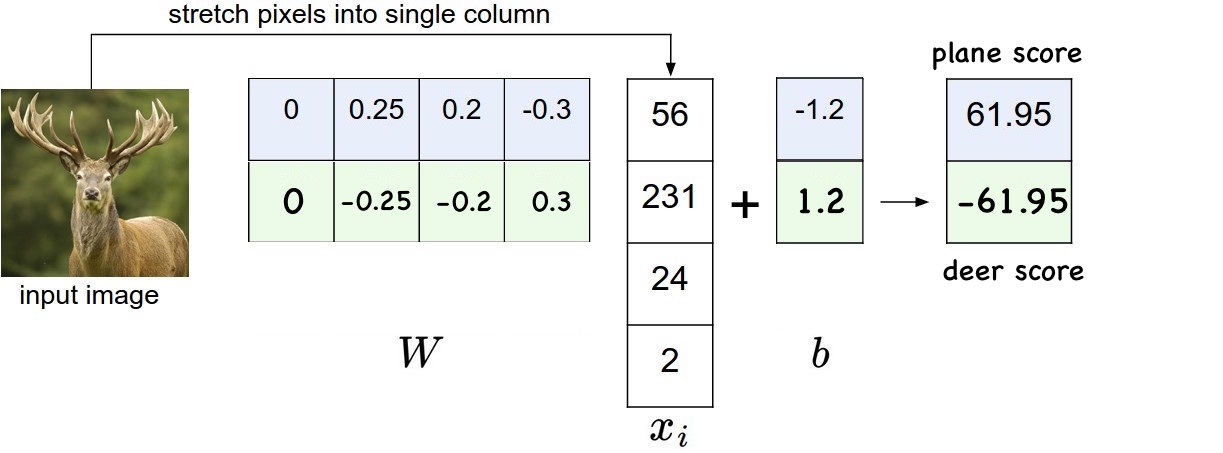
\includegraphics[scale=0.15]{img/clf2}
	\end{center}

\end{frame}

\begin{frame}{Linear Models}
	\begin{center}
		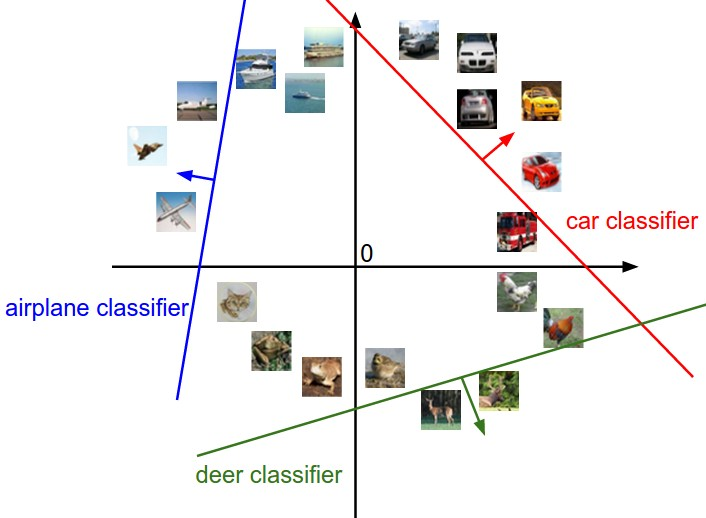
\includegraphics[scale=0.27]{img/pclf3}
		
		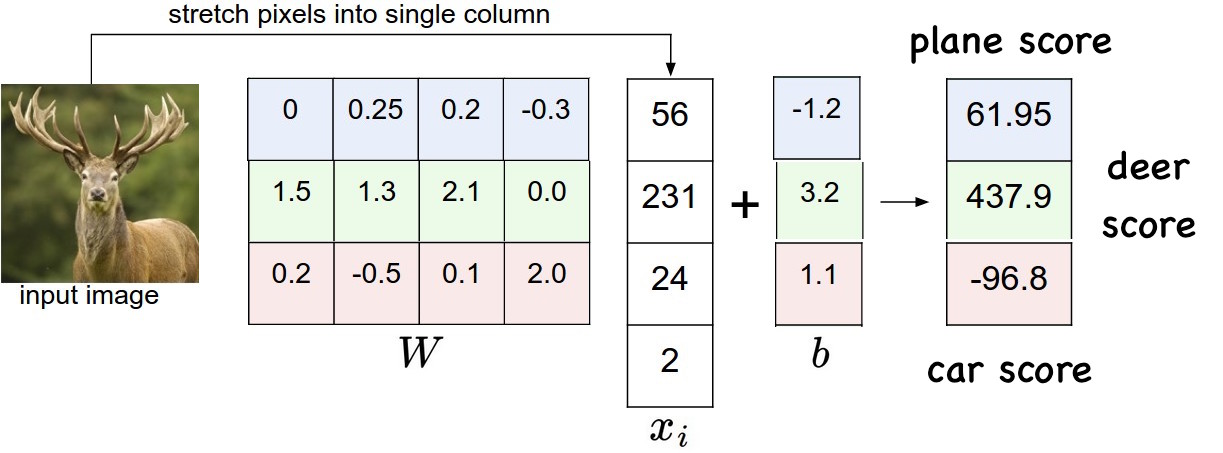
\includegraphics[scale=0.15]{img/clf3}
	\end{center}
	 \href{http://vision.stanford.edu/teaching/cs231n/linear-classify-demo/}{http://vision.stanford.edu/teaching/cs231n/linear-classify-demo/}
\end{frame}

\begin{frame}{Linear Models Plot weights}
	\begin{center}
		  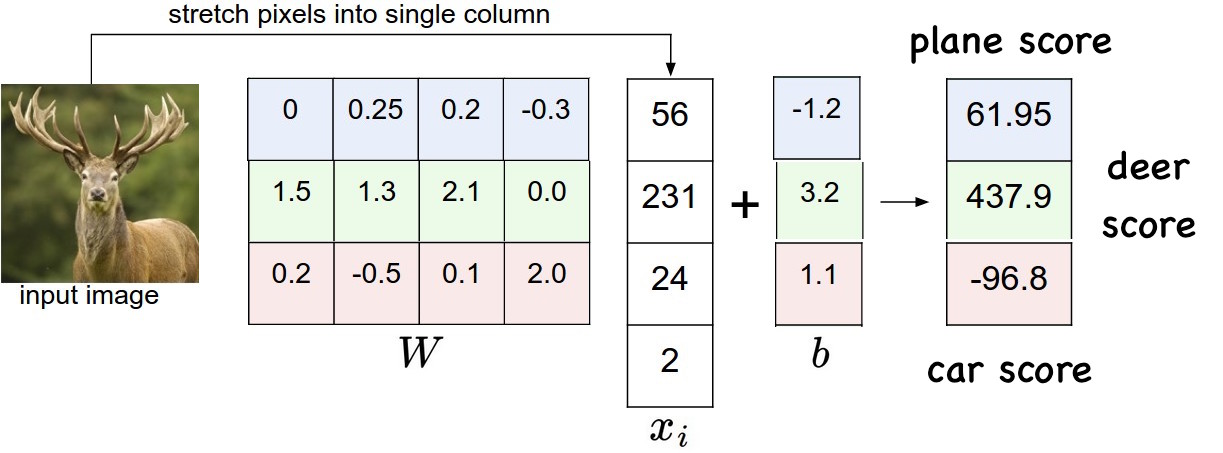
\includegraphics[scale=0.17]{img/clf3}
		
		  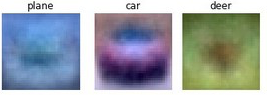
\includegraphics[scale=0.5]{img/w1}
	\end{center}
	\begin{itemize}
		\item    add more classifiers
		  $$score (x) = W_2\cdot(W_1\cdot x + b_1) + b_2 = W\cdot x + b$$
		  it was a bad idea \frownie{} 
		\item    let's add non-linearity
		$$score (x) = W_2\cdot\sigma(W_1\cdot x + b_1) + b_2 \neq W\cdot x + b$$
		  so we made our model more complex \blacksmiley{}
	\end{itemize}
\end{frame}

\begin{frame}{Neural Nets}
			\begin{center}
				  
\includegraphics[scale=0.45]{img/nn1}
				
				  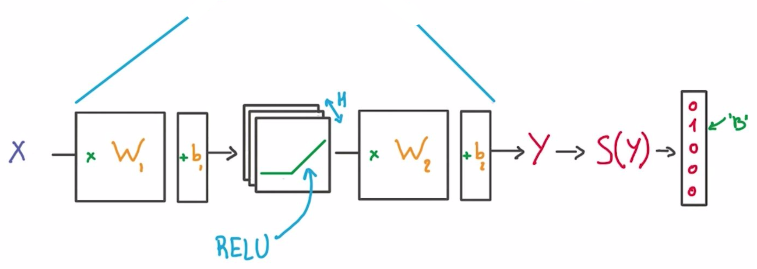
\includegraphics[scale=0.45]{img/nn2}
			\end{center}
			\begin{itemize}
				\item    Back Propagation Idea, evaluate loss gradient by $W_1$ through $W_2$ 
				\item    Layer with linear transformation usually calls Dense or Fully Connected
				\item 	
					  \href{https://goo.gl/77q8Xh}{\textcolor{red}{linear model}} vs 
					            \href{https://goo.gl/ziVfWI}{\textcolor{red}{non-linear}} vs 
					            \href{https://goo.gl/aYiGbl}{\textcolor{red}{deep nonlinear}} 
			\end{itemize}

\end{frame}


\begin{frame}{Recap}
	\begin{itemize}
		  \item In linear models we get only one weight vector per class 
		\begin{center}
			  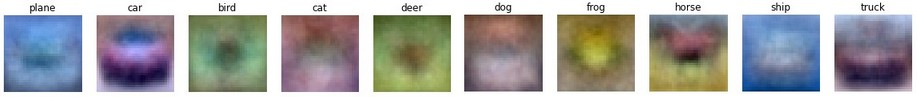
\includegraphics[scale=0.3]{img/w3}
		\end{center}
		\item   Now we got a lot of feature extractor in matrix $W_1$ we call it Fist Layer
		\begin{center}
			  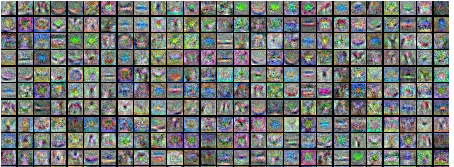
\includegraphics[scale=0.7]{img/w4}
		\end{center}
				
		
	\end{itemize}
\end{frame}

\begin{frame}{Layers}
	\begin{figure}[htbp]
		\centering
		  
		\begin{subfigure}[b]{0.45\textwidth}
			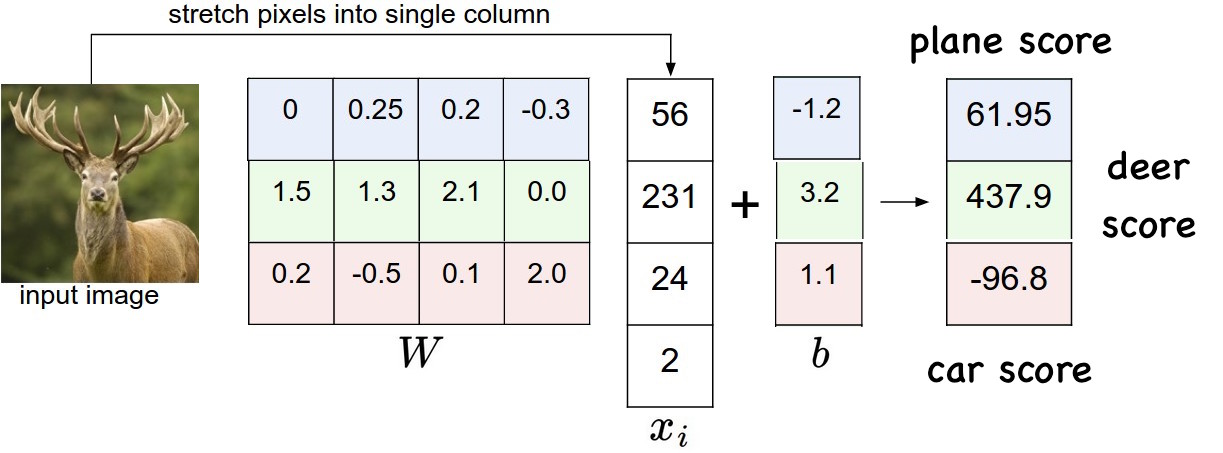
\includegraphics[width=\textwidth]{img/clf3}
			\caption{Dense}
		\end{subfigure}
		  
		\begin{subfigure}[b]{0.45\textwidth}
			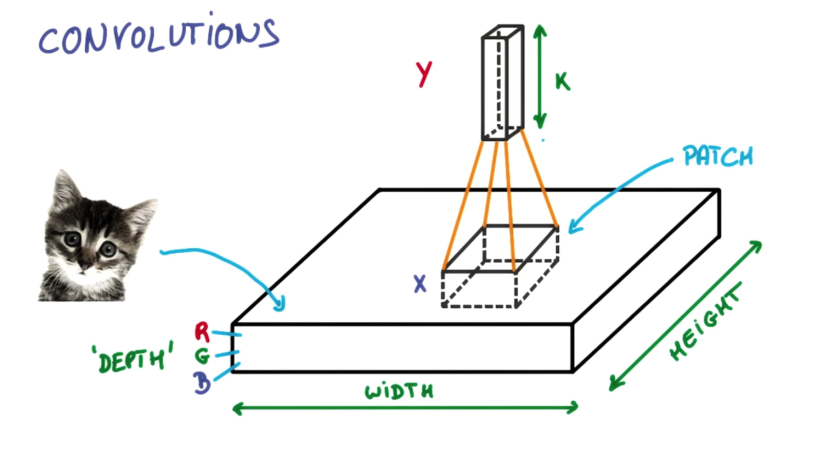
\includegraphics[width=\textwidth]{img/cnn2}
			\caption{\href{	https://bamos.github.io/data/2016-08-09/padding_strides.gif}{Convolution}}
		\end{subfigure}
		
		  
		\begin{subfigure}[b]{0.45\textwidth}
			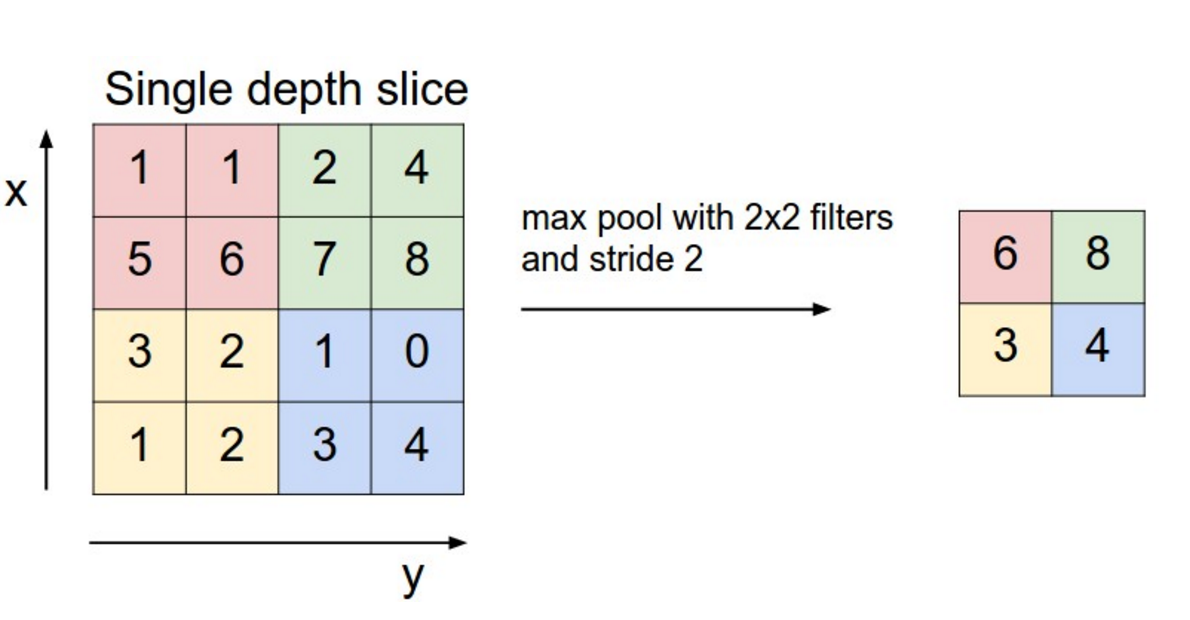
\includegraphics[width=\textwidth]{img/pool}
			\caption{Pooling}
		\end{subfigure}
		  
		\begin{subfigure}[b]{0.4\textwidth}
			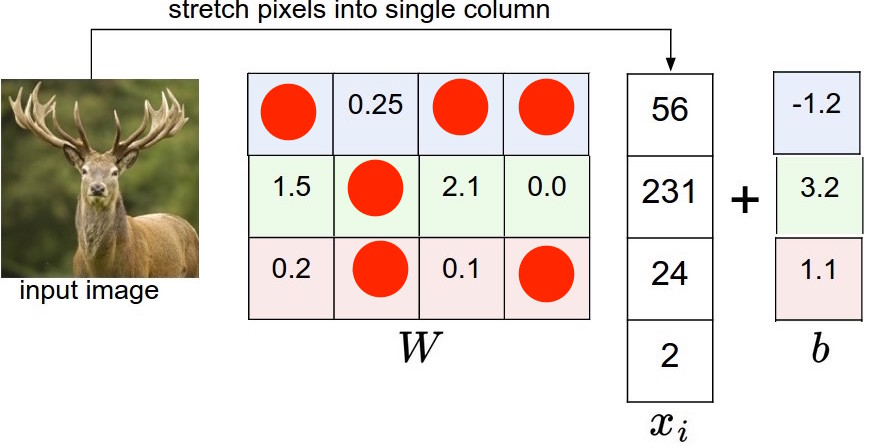
\includegraphics[width=\textwidth]{img/do}
			\caption{Drop Connection}
		\end{subfigure}
		
	\end{figure}
\end{frame}

\begin{frame}{Conv Neural Nets}
	\begin{itemize}
		\item   Too many parameters for each deer position
		\item   We can evaluate local features
		\item   Convolution \href{https://bamos.github.io/data/2016-08-09/padding_strides.gif}{animation}
		\item   Convolution Neural Net
			  \begin{center}
				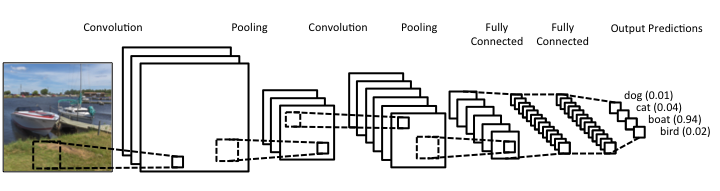
\includegraphics[scale=0.4]{img/cnn}
			\end{center} 

		\item   Good Representation
			 \begin{center}
				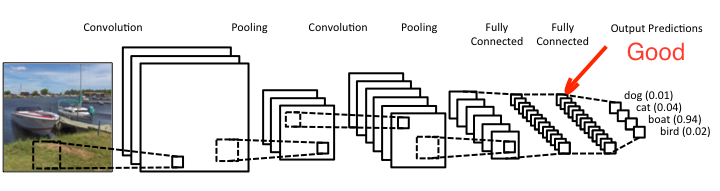
\includegraphics[scale=0.4]{img/cnn_gr}
			\end{center} 
		\item  \href{http://cs.stanford.edu/people/karpathy/cnnembed/}{\textcolor{red}{	http://cs.stanford.edu/people/karpathy/cnnembed/}}
	\end{itemize}
	
	
\end{frame}

\begin{frame}{Aauto-encoders}
	
	\begin{itemize}
		\item   What you should do if there are no training labels?
		\item   We still want to understand smth about images?
		\item   Fully Contented Auto-encoder
			\begin{center}
				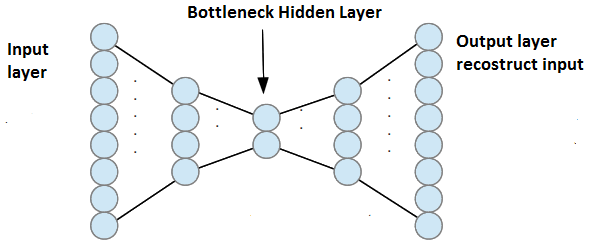
\includegraphics[scale=0.5]{img/autoencoders.png}
			\end{center} 
								
		\item    Convolution Auto-encoder
			\begin{center}
				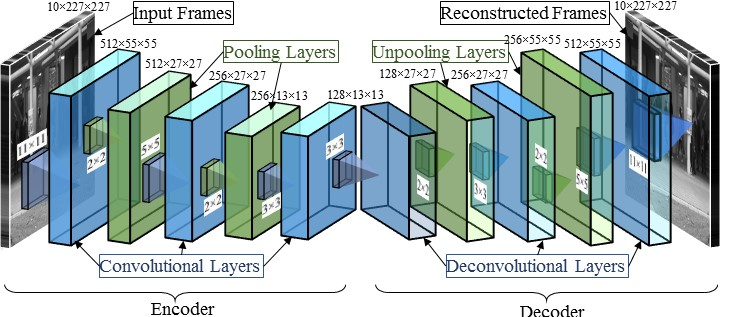
\includegraphics[scale=0.3]{img/cautoenc}
			\end{center} 
	\end{itemize}

\end{frame}

\begin{frame}{Nonlinearities}
	\begin{itemize}
		\item   Activation function
			\begin{center}
				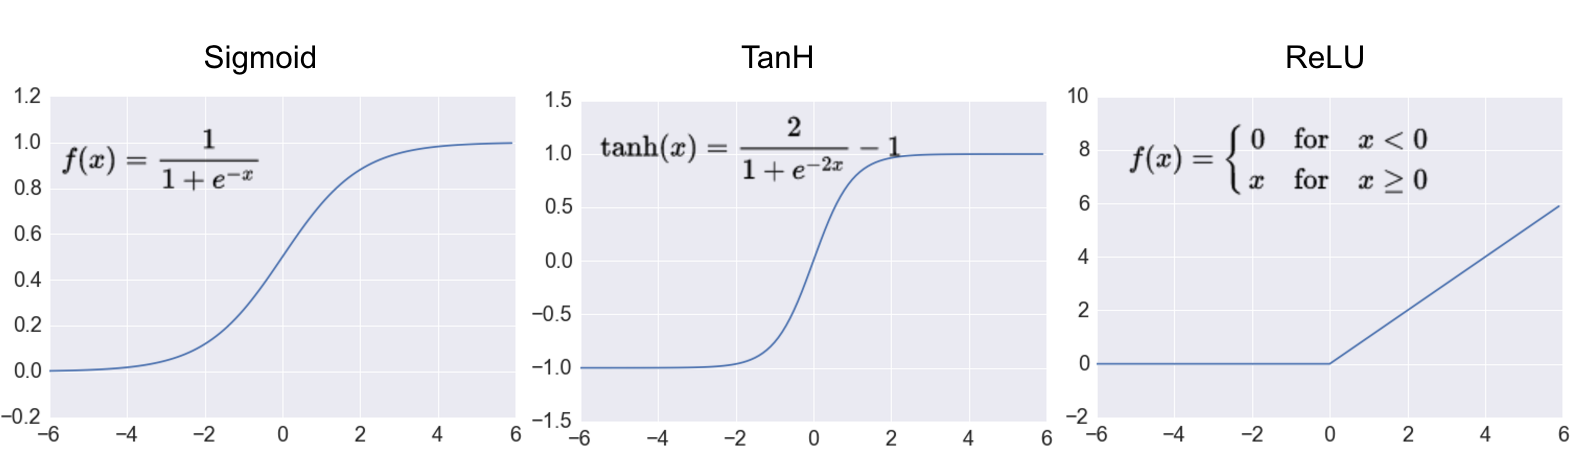
\includegraphics[scale=0.2]{img/act}
			\end{center} 
		\item    From scores to probabilitys -- SoftMax
			\begin{center}
				 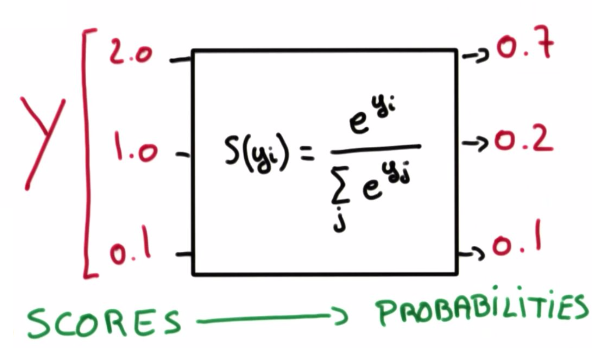
\includegraphics[scale=0.2]{img/sm}
			\end{center}
		\item    Large list is available hear \href{http://lasagne.readthedocs.io/en/latest/modules/nonlinearities.html\#module-lasagne.nonlinearities}{lasagne.nonlinearities} 
	\end{itemize}
\end{frame}



\begin{frame}{Loss Function}
	\begin{itemize}
		\item For regression task and Auto-encoders you can use MSE
			  $$L(\mathbf{y}, \mathbf{\hat{y}}) = (\mathbf{y}-\mathbf{\hat{y}})^2.mean()$$
			
		\item   For classification Cross-Entropy or LogLoss
		  $$LogLoss = -(y_i log(\hat{y}_i)  +(1 - y_i) log(1 - \hat{y}_i))$$
		  $$CE= -\sum_i y_i\, \log \hat{y}_i$$
		\item   For classification Hinge-Loss or SVM \blacksmiley{}
		  $$SVM = ~~~~max(0, - y \cdot \hat{y} + c)$$
		  $$Hinge = \sum_{i \neq y_i} max(0, \hat{y}_i - \hat{y}_{y_i} + c)$$
		\item   You can make loss by yourself 
	\end{itemize}
\end{frame}

\begin{frame}{Optimizers}

	\begin{itemize}
		\item   Stochastic Optimization, we cant eval our function and it's grad
		\item   Stochastic Gradient Decent, so we will compute unbiased estimation
		$$w = w - \alpha \frac{\partial \hat{L}}{\partial w}$$
		\item   Stochastic Gradient Decent with Momentum
			\begin{center}
				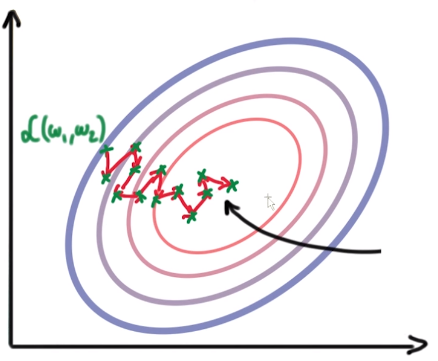
\includegraphics[scale=0.2]{img/mom}
			\end{center} 
		\item    Stochastic Gradient Decent with Momentum and Rescaling (adam)
			\begin{center}
				  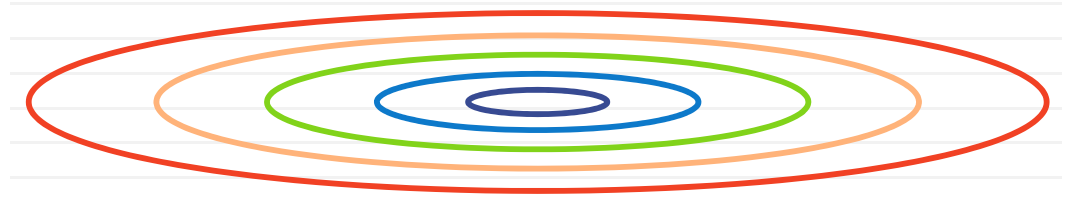
\includegraphics[scale=0.2]{img/bs}
			\end{center} 
		
	\end{itemize}
	  \href{http://sebastianruder.com/content/images/2016/09/contours_evaluation_optimizers.gif}{\textcolor{red}{contours evaluation optimizers}}, 
	\href{http://sebastianruder.com/content/images/2016/09/saddle_point_evaluation_optimizers.gif}{\textcolor{red}{saddle point}}
	
\end{frame}

\begin{frame}{ImagNet Challenge}
	\begin{itemize}
		\item   Imagnet		
		
		\begin{center}
			
\includegraphics[scale=0.2]{img/imn}
		\end{center} 

		\item   Errors-Number of Layers Plot vs Time 
		\begin{center}
			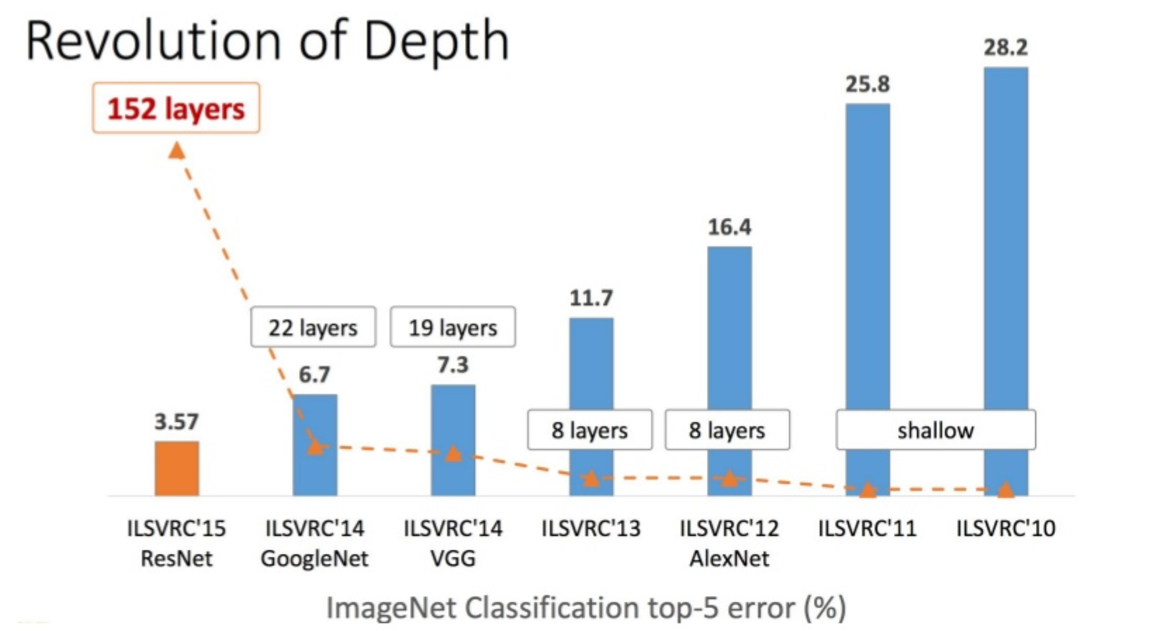
\includegraphics[scale=0.2]{img/dr}
		\end{center} 
			\end{itemize}
		plot credit: Kaiming He
\end{frame}

\begin{frame}{Popular architectures}
		\begin{center}
			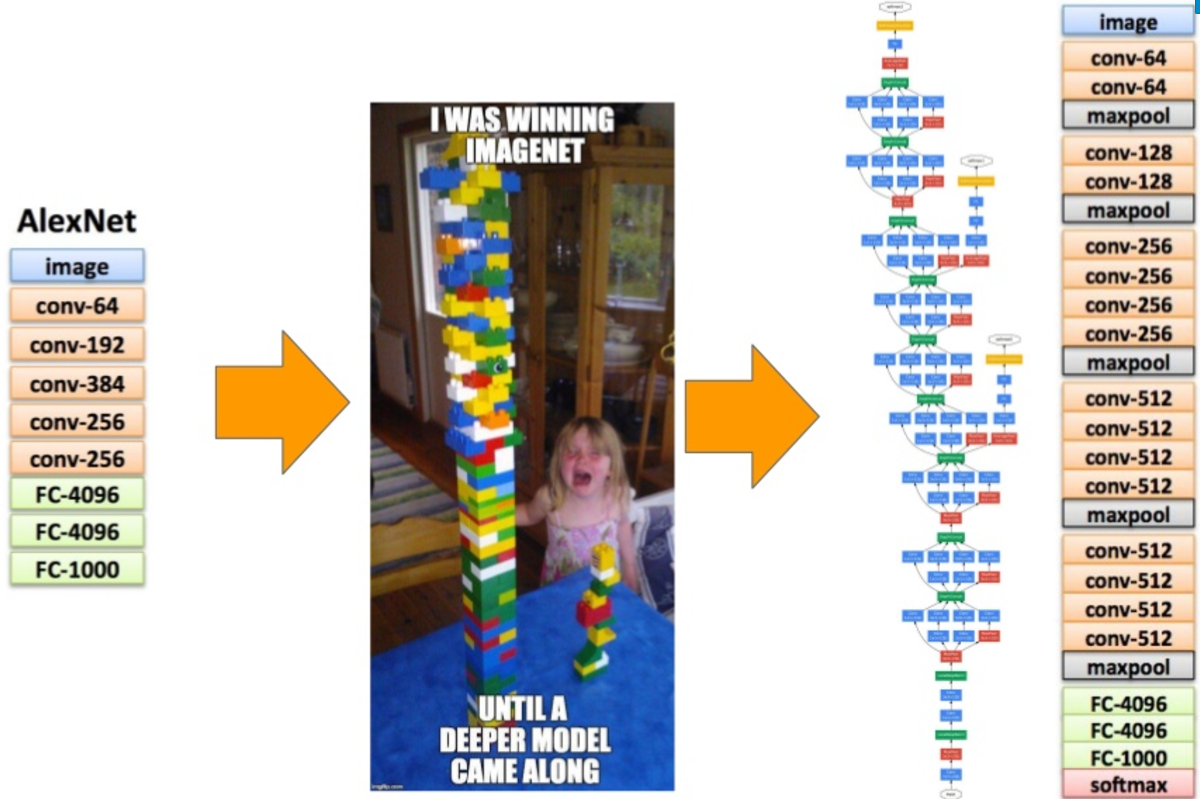
\includegraphics[scale=0.23]{img/im2}
		\end{center} 
\end{frame}

\begin{frame}{Popular architectures}
	\begin{center}
		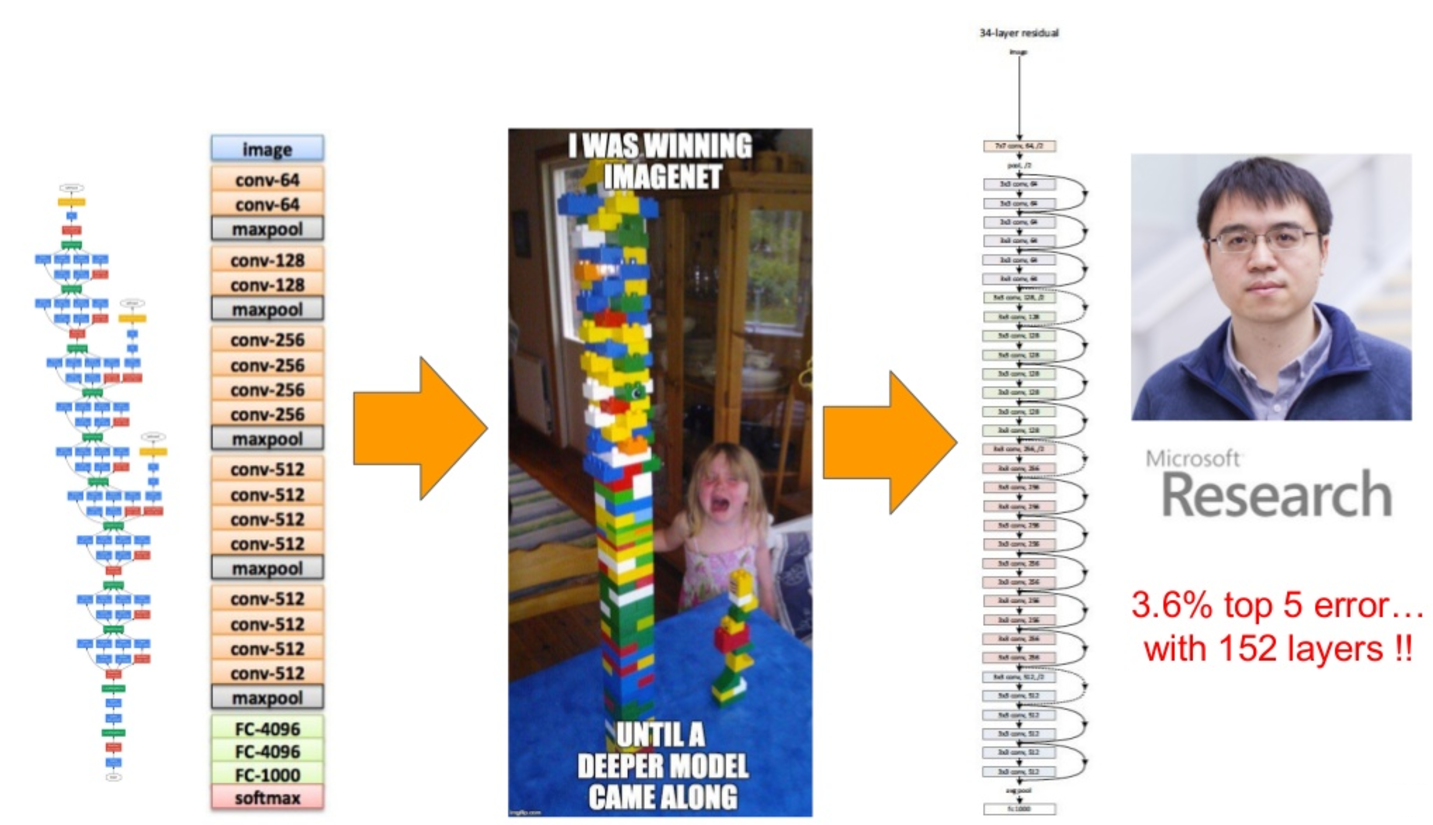
\includegraphics[scale=0.23]{img/im1}
	\end{center} 
\end{frame}

\begin{frame}[fragile]{Code should be like this}
	 
\begin{minted}{python}
from lasagne import layers as ll
\end{minted}
 
\begin{minted}{python}
nn = ll.InputLayer(shape=(None, 1, 28, 28), input_var)
\end{minted}
 
\begin{minted}{python}
nn = ll.Conv2DLayer(nn, num_filters=32, filter_size=5)
nn = ll.MaxPool2DLayer(nn, pool_size=(2, 2))
\end{minted}
 
\begin{minted}{python}
nn = ll.DropOutLayer(nn, 0.5)
nn = ll.DenseLayer(nn, 10, nonlinearity=softmax)
\end{minted}
 
\begin{minted}{python}
loss = crossentropy(ll.get_output(nn), target_var).mean()
\end{minted}
 
\begin{minted}{python}
params = ll.get_all_params(nn, trainable=True)
updates = lasagne.updates.adam(loss, params)
\end{minted}
\end{frame}

\begin{frame}{Recap}
	
 	Recap:
	\begin{itemize}
		\item Deep Architectures are cool
		\item Use Pre-trained Nets and Fine-tuning for your tasks
		\item Old math doesn't work if a lot of data 
	\end{itemize}
	
	\vspace{1cm}
 	Good courses/books
	\begin{itemize}
		\item \href{https://github.com/Lasagne/Recipes/tree/master/modelzoo}{https://github.com/Lasagne/Recipes/tree/master/modelzoo}
		\item \href{cs231n.stanford.edu}{cs231n.stanford.edu}
		\item \href{udacity.com/course/deep-learning--ud730}{udacity.com/course/deep-learning--ud730}
		\item \href{deeplearningbook.org}{deeplearningbook.org}
	\end{itemize}
\end{frame}
\begin{frame}{} 
	\begin{center}				
		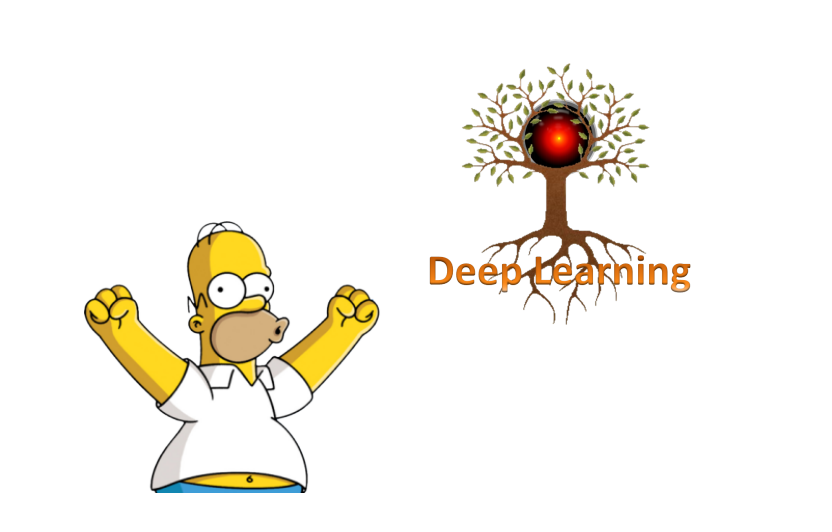
\includegraphics[scale=0.35]{img/csf}
		
		{\huge Current Status of your Field!}

	\end{center}
\end{frame}
\begin{frame}{How to apply ML for Music Data to get Money?} 
	\begin{itemize}
		 \item  Your are working in a big music service as a data scientist
		\begin{center}		  
			 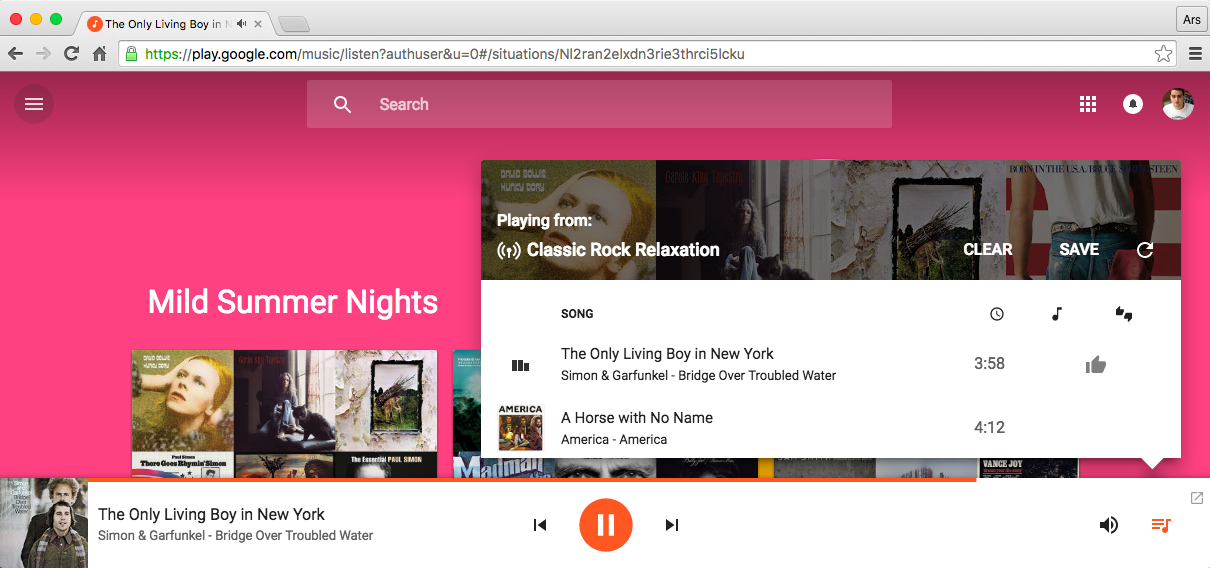
\includegraphics[scale=0.15]{img/interface}~~~  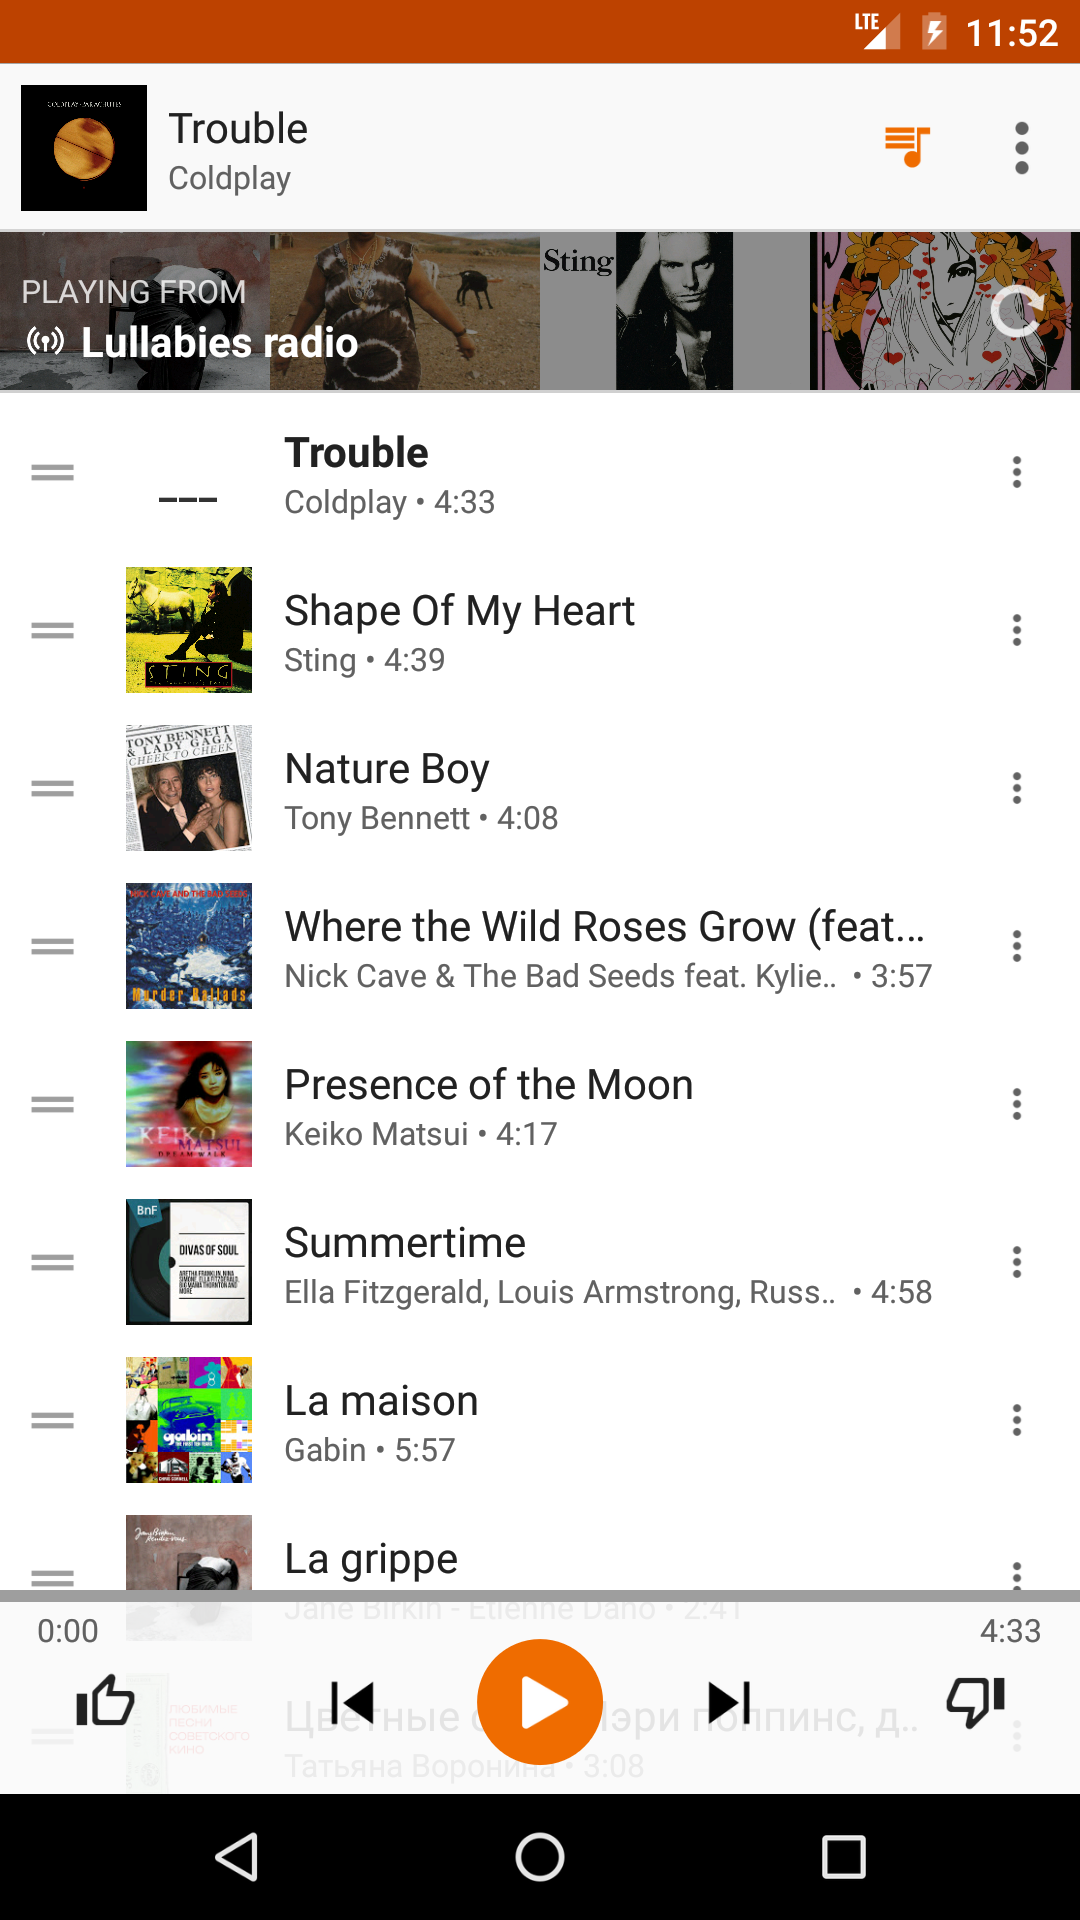
\includegraphics[scale=0.044]{img/phone}
		\end{center}
		 \item   In this service there's a lot of music data -- mp3 files
		\begin{center}
			 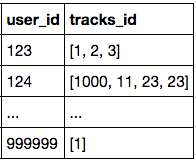
\includegraphics[scale=0.4]{img/u2t}~~~~  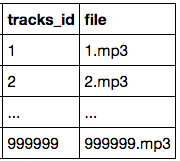
\includegraphics[scale=0.4]{img/t2f} 
		\end{center}
		 \item   You were given the task -- make money using this data
	\end{itemize}
\end{frame}

\begin{frame}{What is the sound?} 
	\begin{itemize}
		\item     Waves and Recording
		\begin{center}		  
			 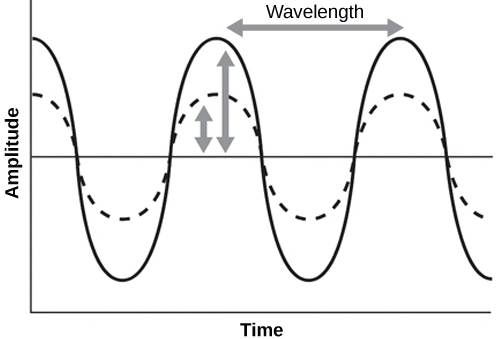
\includegraphics[scale=0.25]{img/wave} ~~~    	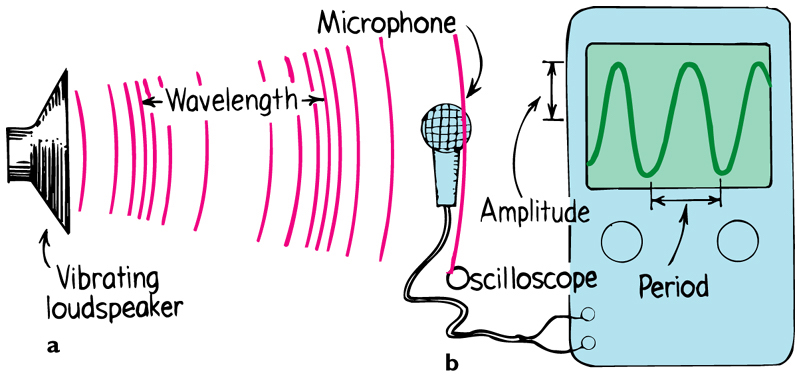
\includegraphics[scale=0.2]{img/sound}
		\end{center}
		\item     How to store sound? Store as big-big array with sampling frequency
		\begin{center}
			 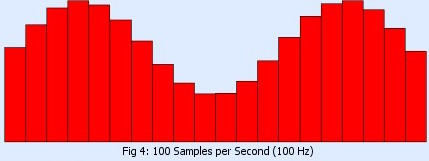
\includegraphics[scale=0.35]{img/sf1}~~~~   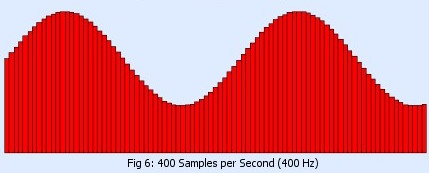
\includegraphics[scale=0.35]{img/sf2} 
		\end{center}
		\item    $[1, 2, 3, 5, 3, 2, 1, 1, 1, 1, 2, 3, 5, 3, 2]$,   Usually 16 000 float per second
	\end{itemize}
\end{frame}

\begin{frame}{Finding similar tracks}
	\begin{itemize}
		\item     How to find similar tracks using ML methods?
		\begin{center}		  
			   \textcolor{blue}{Data}: 30 sec * 16000 features, $10^7$ items
			
			   \textcolor{red}{Task}: define function of $similarity(track_i, track_j)$
		\end{center}
		
		\item         Why ordinary methods are so bad?
		\begin{itemize}
			\item      shift and noise tolerance, over-fitting 
		\end{itemize}
		
		\item      Metric approach is still good idea, if we have a high level description
		\item      Good representation of music track
		\begin{itemize}
			\item      Human -- guitar, rock, Queen, 1997, UK, 3 min., .... 
			\item      Computer -- good small vector of numbers  
		\end{itemize}
		
		\begin{center}
			   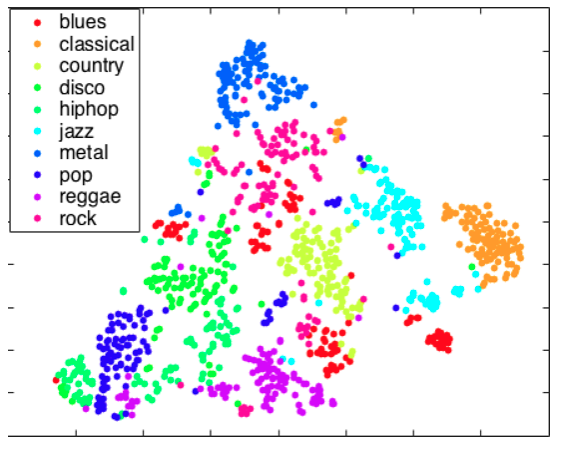
\includegraphics[scale=0.2]{img/geners}
		\end{center}
		
	\end{itemize}
\end{frame}


\begin{frame}{Get good representation using Neural Nets}
	\begin{center}
	   	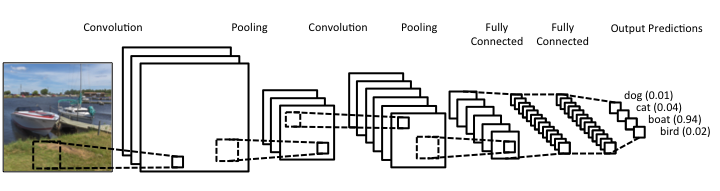
\includegraphics[scale=0.4]{img/cnn}
		
	   	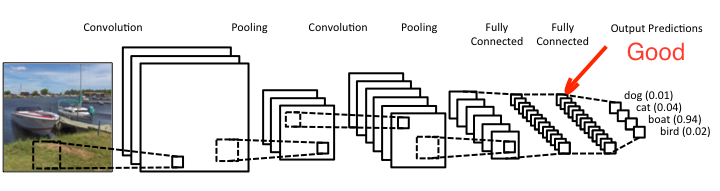
\includegraphics[scale=0.4]{img/cnn_gr}
	\end{center}
	 
	\begin{tcolorbox}[colback=gray!2, colframe=red!90, title=Problem]
		  \centering We need to get picture!
	\end{tcolorbox}
\end{frame}

\begin{frame}{What is the sound part 2?} 
	We have some wave 
	
	\begin{center}
		   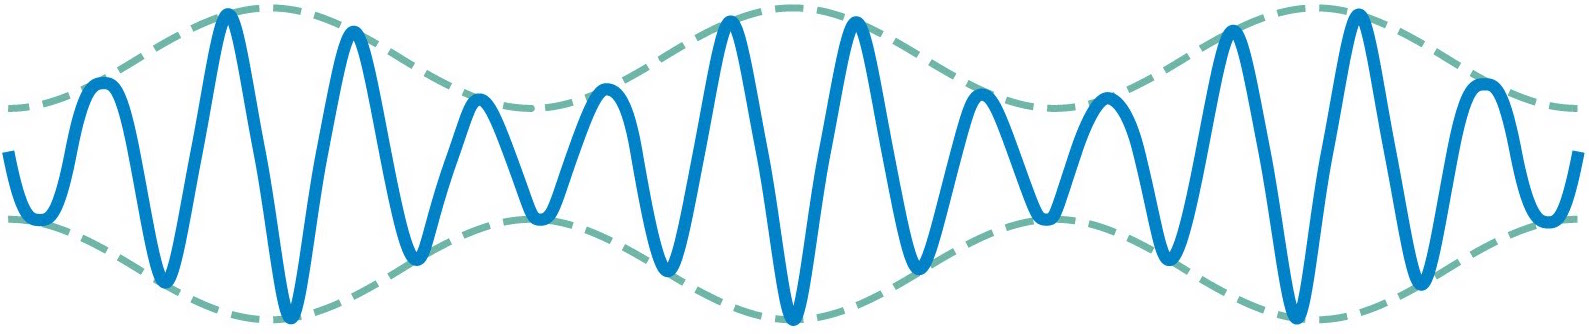
\includegraphics[scale=0.1]{img/wave1}
	\end{center}
	
	   represent wave as a sum of two waves 
	
	\begin{center}
		   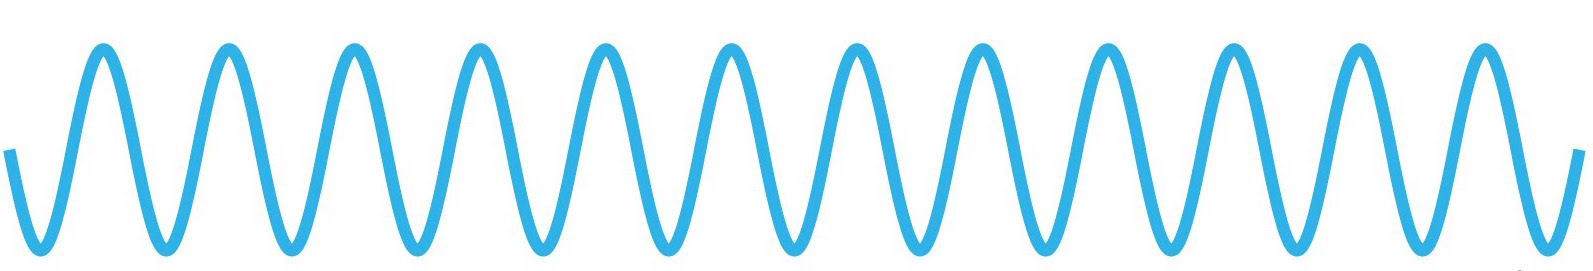
\includegraphics[scale=0.1]{img/wave2}
		   
\includegraphics[scale=0.1]{img/wave3}
	\end{center}
	
	   sound is a combination of big waves range
	
	\begin{center}
		   \includegraphics[scale=0.4]{img/sound_}
	\end{center}
	
	\begin{center}
		   What we lost in our representation?
	\end{center}	
\end{frame}

\begin{frame}{What is the sound part 2? Get Frequency} 
	\begin{center}
		   \includegraphics[scale=0.5]{img/sound_sl}
		
		   \includegraphics[scale=0.4]{img/hist}~~~~~~~~
		
		   \includegraphics[scale=0.4]{img/histc}~~~~~~~~~
		
		    \includegraphics[scale=0.3]{img/spect}~~~~~~~~~
	\end{center}
	
\end{frame}


\begin{frame}{We need to train Neural Nets, but how can we do that?!}
	\begin{itemize}
		\item      But how can we train nets on music? 
		\item      Let's invent a fake machine learning task
		
		\includegraphics[scale=0.4]{img/cnn_what2predict}~~~~~~~~~
		
		\begin{itemize}
			\item      genre classification
			\item      artist classification
			\item      rating prediction
			\item      .....
		\end{itemize}
	\end{itemize} 
	
\end{frame}

\begin{frame}{Fully connected NN} 
	\begin{center}
		   \includegraphics[scale=0.5]{img/fc}
	\end{center}
	\begin{itemize}
		\item      too many parameters -- number of weights = $16^4 * neurons$ + ... 
		\item      It doesn't work =( 
	\end{itemize}
\end{frame}

\begin{frame}{Convolution NN} 
	   Let's invent some convolution architecture
	\begin{center}
		   \includegraphics[scale=0.5]{img/conv}
	\end{center}
	   important detail -- pooling of time axis \href{http://bit.ly/1slJTgi}{[\textcolor{green}{Spotify )))} Deep Learning]}
	\begin{center}				
		   \includegraphics[scale=1.5]{img/rconv}
	\end{center}
\end{frame}

\begin{frame}{How to measure quality of good representation?} 
	   What we have?
	\begin{itemize}
		\item      We have represented each track as a vector
		\item      But maybe our solution is too bad, how can we understand that?
		\item      How to test "good representation"?
	\end{itemize}
	
	   Let's invent the metrics:
	\begin{itemize}
		\item      by hand
		\item      using assessors
		\item      recommendation quality 
		\item      using vectors to classify another labels
	\end{itemize}
\end{frame}

\begin{frame}{Let's adapt to Different length and Additional information} 
	   How to use any length?:
	\begin{enumerate}
		\item      Average prediction for many patches 		
		\item      Recurrent neural net on many patches
		\begin{center}				
			   \includegraphics[scale=0.25]{img/rnn}
		\end{center} 
		\item      Whatever?
	\end{enumerate}
	   How to take account?:
	\begin{enumerate}
		\item      Lyrics
		\begin{center}
		   	Concat(TextRNN, Conv) $\rightarrow$ FC $\rightarrow$ Cost
		\end{center}
		\item      Genre, Artist, Year    -- embedding too, multi-cost task
		\item      ....
	\end{enumerate}
\end{frame}

\begin{frame}{} 
	\begin{center}				
		\includegraphics[scale=0.35]{img/csf}
		
		{\huge Current Status of your Field!}
		
		Thanks for your attention!
	\end{center}
\end{frame}

\end{document}